\chapter{Tool demonstration: Transatomic Power MSR}

In this chapter, I demonstrate SaltProc v1.0 capabilities for the \gls{TAP} 
\gls{MSR}. The \gls{TAP} concept was selected because it is well analyzed in 
the literature \cite{betzler_two-dimensional_2017, betzler_assessment_2017-1};
thus, code-to-code verification with ChemTRITON/SCALE is possible 
\cite{betzler_assessment_2017-1}. The demonstration was performed for two 
timescales:
\paragraph{Long-term.} I performed the \gls{TAP} \gls{MSR} core lifetime-long 
(25 years) depletion simulation with moderate time resolution (3-day depletion 
step) and constant, 100\% power level. The 
results obtained with SaltProc v1.0 are compared with recent efforts discussed 
in Chapter 1, more specifically with full-core \gls{TAP} depletion analysis 
with ideal removal efficiencies by Betzler \emph{et al.}  
\cite{betzler_assessment_2017-1}. This validation effort showed that SaltProc 
v1.0 solution is correct for the case with \emph{ideal extraction efficiency}.
\paragraph{Short-term (transient).} I performed the 24-hour-long depletion 
simulation with changing, load following reactor power with the fine time 
resolution (variable depletion step from 1 to 30-min). The depletion 
calculation for the \gls{TAP} in load following regime capture the effects of 
xenon poisoning and evaluate the benefit of using an online gas removal system.

In this chapter, I also analyze the reactor load-following capability for 
various moderator configurations and fuel salt compositions to bound design 
parameters of gas removal system to ensure load-following operation. 

\section{Transatomic Power Molten Salt Reactor concept design and model  
description}

The \gls{TAP} concept is a 1250 MW$_{th}$ \gls{MSR} with a LiF-based uranium 
fuel salt \cite{transatomic_power_corporation_technical_2016}. This concept 
uses configurable zirconium hydride rods as the moderator while most \gls{MSR} 
designs typically propose high-density reactor graphite. Zirconium hydride 
offers a much higher neutron moderating density than graphite: much less 
zirconium hydride volume is needed to achieve a thermal energy spectrum 
similar to one obtained with graphite moderator. Moreover, zirconium hydride 
has a much longer lifespan in extreme operational conditions (high 
temperature, large neutron flux, chemically aggressive salt) than reactor 
graphite. Finally, zirconium hydride is a nonporous material and holds up 
fewer neutron poisons (e.g., xenon, krypton) than does high-density 
reactor graphite.

In this section, the design characteristics and reprocessing plant design are 
based on information presented in the TAP white papers  
\cite{transatomic_power_corporation_technical_2016,
transatomic_power_corporation_neutronics_2016} and \gls{ORNL} technical 
reports \cite{betzler_two-dimensional_2017, betzler_assessment_2017-1}.

\subsection{TAP design description}

Figure~\ref{fig:tap-rendering} demonstrates a rendering of the primary and 
secondary loop of the \gls{TAP} \gls{MSR} seated inside a concrete nuclear 
island. Figure~\ref{fig:tap-primary-scheme} shows the schematic design of a 
520 MW$_{e}$, 2-loop nuclear reactor system with an intermediate salt loop.
\begin{figure}[h] % replace 't' with 'b' to 
	\centering
	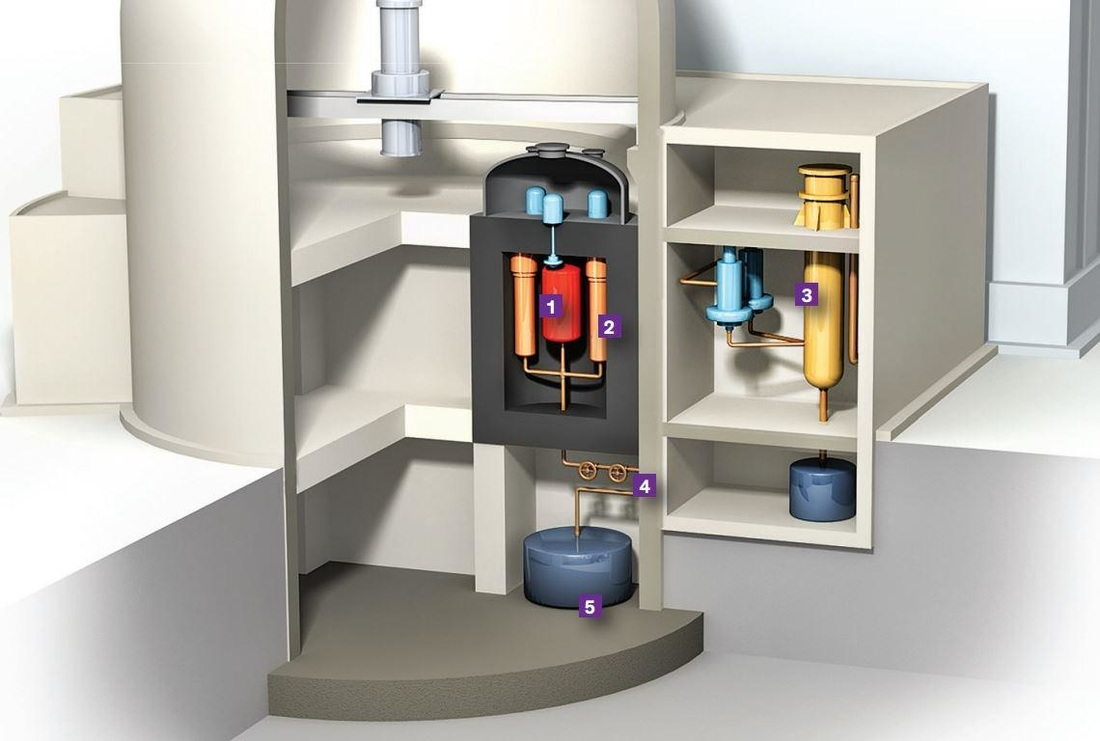
\includegraphics[width=\textwidth]{ch4/tap_render.jpg}
	\caption{Rendering of the \gls{TAP} \gls{MSR}. The fission happens in the 
		fuel salt inside the reactor vessel (1). The heat generated by 
		self-sustaining nuclear fission reaction would be transferred to the 
		secondary salt by heat exchanger (2), which would boil water in the 
		steam 
		generator (3). Valves made of salt with higher melting point (4) would 
		melt in case of emergency, allowing the salt to drain into a drain 
		tank 
		(5) which is able to passively dissipate decay heat	(reproduced from 
		\cite{strickland_transatomic_2014}, illustration by Emily Cooper).}
	\label{fig:tap-rendering}
\end{figure}
\begin{figure}[h] % replace 't' with 'b' to 
	\centering
	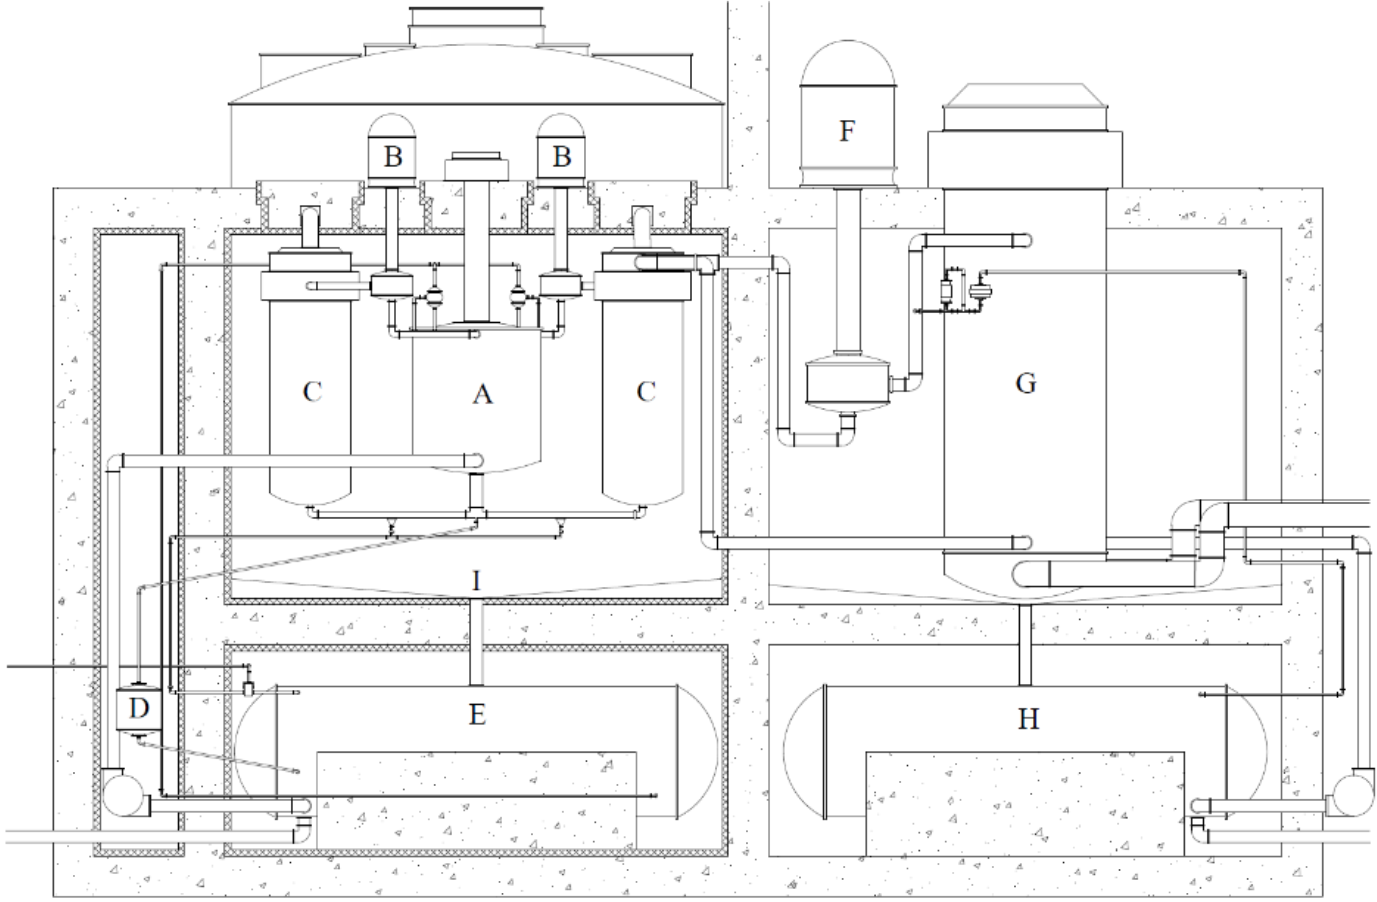
\includegraphics[width=\textwidth]{ch4/tap_simplified_scheme.png}
	\caption{Simplified schematic of the \gls{TAP} \gls{MSR} primary and  
		secondary loops (reproduced from the Transatomic Power Technical White 
		Paper \cite{transatomic_power_corporation_technical_2016}). Figure 
		legend: 
		A) reactor vessel, b) fuel salt pumps, C) primary heat exchangers, D) 
		freeze plug, E) primary loop drain tank, F) secondary loop salt pump, 
		G) 
		steam generator, H) secondary loop drain tank, I) fuel catch basin.}
	\label{fig:tap-primary-scheme}
\end{figure}

The \gls{TAP} design (figure~\ref{fig:tap-side-view}) is very similar to 
original \gls{MSRE} design developed by \gls{ORNL} 
\cite{haubenreich_experience_1970} but has two major innovations: 
the fuel salt composition and the moderator. The \gls{MSRE}'s 
LiF-BeF$_2$-ZrF$_4$-UF$_4$ salt has been substituted with LiF-UF$_4$ salt 
which allows for an increase in the uranium concentration within the fuel salt 
from 0.9 to 27.5\% while maintaining a relatively low melting point 
(490$^{\circ}$C compared with 434$^{\circ}$C for the original \gls{MSRE}'s 
salt) \cite{betzler_two-dimensional_2017}. The graphite has a very high 
thermal scattering cross section which makes it a perfect moderator but has 
a few major drawbacks: 
\begin{enumerate}[label=(\alph*)]
	\item low lethargy gain per collision requires a large volume of 
	moderator to be present to reach criticality, which leads to a larger core 
	and obstructs the core power density;
	\item even special reactor-grade graphite has relatively high porosity, 
	consequently, it holds gaseous \glspl{FP} (e.g., tritium, xenon) in pores;
	\item reactor graphite lifespan in a commercial reactor is 
	approximately 10 years \cite{robertson_conceptual_1971}.
\end{enumerate}
As previously mentioned, to resolve these issues, the \gls{TAP} concept uses 
zirconium hydride instead of graphite, allowing for a more compact core and a 
significant increase in power density. These two innovative design choices, 
together with a configurable moderator (the moderator-to-fuel ratio can be 
changed during operation), facilitate the deployment of this conceptual design 
in the current commercially available 5\% enriched \gls{LEU} fuel cycle. 
\begin{figure}[h] % replace 't' with 'b' to 
	\hspace{+2.2in}
	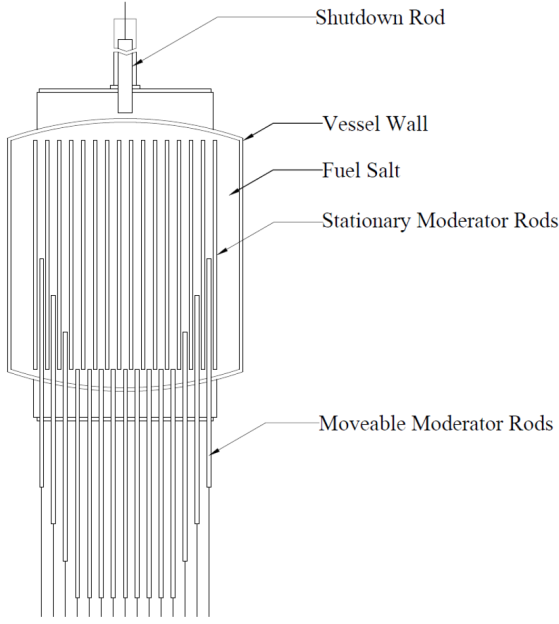
\includegraphics[width=0.65\textwidth]{ch4/tap_front_view.png}
	\caption{The \gls{TAP} \gls{MSR} schematic view showing movable moderator 
		rod bundles and shutdown rod (reproduced from Transatomic Power 
		White Paper \cite{transatomic_power_corporation_technical_2016}).}
	\label{fig:tap-side-view}
\end{figure}

The \gls{TAP} \gls{MSR} primary loop contains the reactor core volume  
(including the zirconium hydride moderator rods with silicon carbide  
cladding), pumps, and primary heat exchangers. Pumps circulate the  
LiF-(Act)F$_4$ fuel salt through the primary loop. The pumps, vessels, tanks, 
and piping are made of a nickel-based alloy (similar to Hastelloy-N\footnote{ 
Hastelloy-N is very common in \gls{MSR} concepts now, but was developed at 
\gls{ORNL} in the \gls{MSRE} program that started in the 1950s.}), which 
is highly resistant to corrosion in various molten salt environments. Inside 
the reactor vessel, near the zirconium hydride moderator rods, the fuel salt 
is in a critical configuration and generates heat. Table~\ref{tab:tap_tab} 
contains details of the \gls{TAP} system design which are taken from technical 
white paper \cite{transatomic_power_corporation_technical_2016} and a 
neutronics overview \cite{transatomic_power_corporation_neutronics_2016} as 
well as \gls{ORNL} analysis of the \gls{TAP} design 
\cite{betzler_two-dimensional_2017, betzler_assessment_2017-1}. 
%%%%%%%%%%%%%%%%%%%%%%%%%%%%%%%%%%%%%%%%
\begin{table}[h!]
	\caption{Summary of principal data for the \gls{TAP} \gls{MSR} 
		(reproduced from \cite{betzler_assessment_2017-1, 
		transatomic_power_corporation_technical_2016}). }
	\begin{tabularx}{\textwidth}{ s  s}
		\hline
		Thermal power   		& 1250 MW$_{th}  $       		\\ 
		Electric power		    & 520 MW$_e  $ 			 		\\ 
		Gross thermal efficiency& 44\%     				 		\\  
		Outlet temperature      & 620$^{\circ}$C         		\\ 
		Fuel salt components    & LiF-UF$_4$				    \\  
		Fuel salt composition   & 72.5-27.5 mole\%				\\  
		Uranium enrichment      & 5\% $^{235}$U          	    \\
		Moderator               & Zirconium Hydride (ZrH$_{1.66}$) rods \\
								& (with silicon carbide cladding)       \\
		Neutron spectrum        & intermediate at the \gls{BOL}             \\
		                        & thermal at the \gls{EOL}			\\
		\hline
	\end{tabularx}
	\label{tab:tap_tab}
\end{table}
%%%%%%%%%%%%%%%%%%%%%%%%%%%%%%%%%%%%%%%%%%%%%%%%%%%%%%%%%%%%%%%%%%%%%%%%%%%%%%%

\subsection{TAP core design}
In the \gls{TAP} core (Figure~\ref{fig:tap-core-ben}), fuel salt flows around 
moderator assemblies consisting of lattices of zirconium hydride rods clad in 
a corrosion-resistant silicone carbide. The \gls{TAP} reactor pressure vessel 
is a cylinder with an inner radius 150 cm, height 350 cm, and wall thickness 5 
cm made of a nickel-based alloy. 
\begin{figure}[t] % replace 't' with 'b' to 
	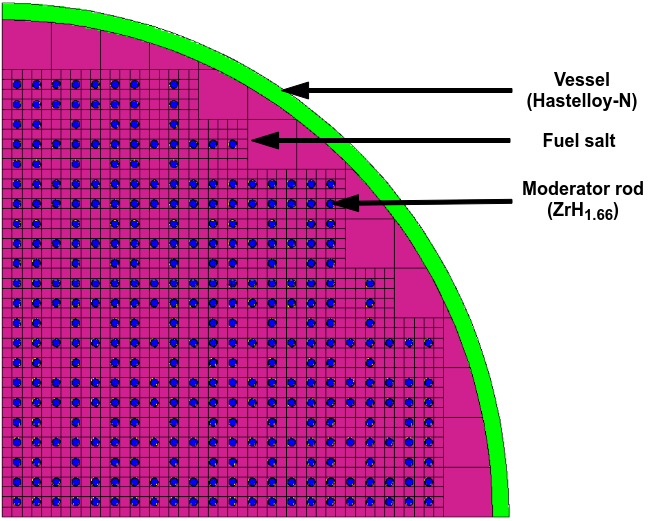
\includegraphics[width=\textwidth]{ch4/tap_core_ornl.png}
	\vspace{-0.35in}
	\caption{The \gls{TAP} \gls{MSR} schematic core view showing moderator 
		rods (reproduced from ORNL/TM-2017/475  
		\cite{betzler_assessment_2017-1}).}
	\label{fig:tap-core-ben}
\end{figure}

The \gls{SVF} in the core is parameter similar to wide-used moderator-to-fuel 
ratio and can be defined as:
\begin{align}
SVF &= \frac{V_F}{V_F+V_M} = \frac{1}{1+V_M/V_F}
\intertext{where}
V_F &= \mbox{the fuel volume $[m^3]$} \nonumber \\
V_M &= \mbox{the moderator volume $[m^3]$} \nonumber \\
V_M/V_F &= \mbox{the moderator-to-fuel salt ratio $[-]$.} \nonumber
\end{align}

Figure~\ref{fig:svf-predetermined} shows the \gls{SVF} variation during  
operation that shifts the reactor neutron energy spectrum from intermediate to 
thermal to maximize fuel burnup. At the \gls{BOL}, a high \gls{SVF} is 
selected to obtain relatively hard spectrum and enhance fertile material 
($^{238}$U) conversion into the fissile material ($^{239}$Pu) while the 
startup fissile material ($^{235}$U) inventory is still large. As fissile 
concentration in the fuel salt declines, an additional moderator are 
introduced to maintain criticality, leading to salt volume fraction decrease 
(see Figure~\ref{fig:svf-predetermined}).

Initial \gls{TAP} concept suggested vary salt volume fraction by inserting 
fixed-sized moderator rods via the bottom of the reactor vessel (for safety 
considerations), similarly to moving the control rods in a \gls{BWR}, as shown 
in Figure~\ref{fig:tap-side-view} 
\cite{transatomic_power_corporation_neutronics_2016}. The later \gls{TAP} 
concept proposes reducing the \gls{SVF} by reconfiguring the moderator rods 
during regular shutdown for reactor maintenance 
\cite{betzler_assessment_2017-1}. For the 
\gls{TAP} reactor, \gls{EOL} occurs when the maximum number of moderator rods 
are inserted into the core, and a further injection of fresh fuel salt does 
not alter criticality. Unmoderated salt is flowing in the annulus between the 
core, and the vessel wall provides for a potential reduction in fast neutron 
flux at the vessel structural material .
\begin{figure}[t] % replace 't' with 'b' to 
	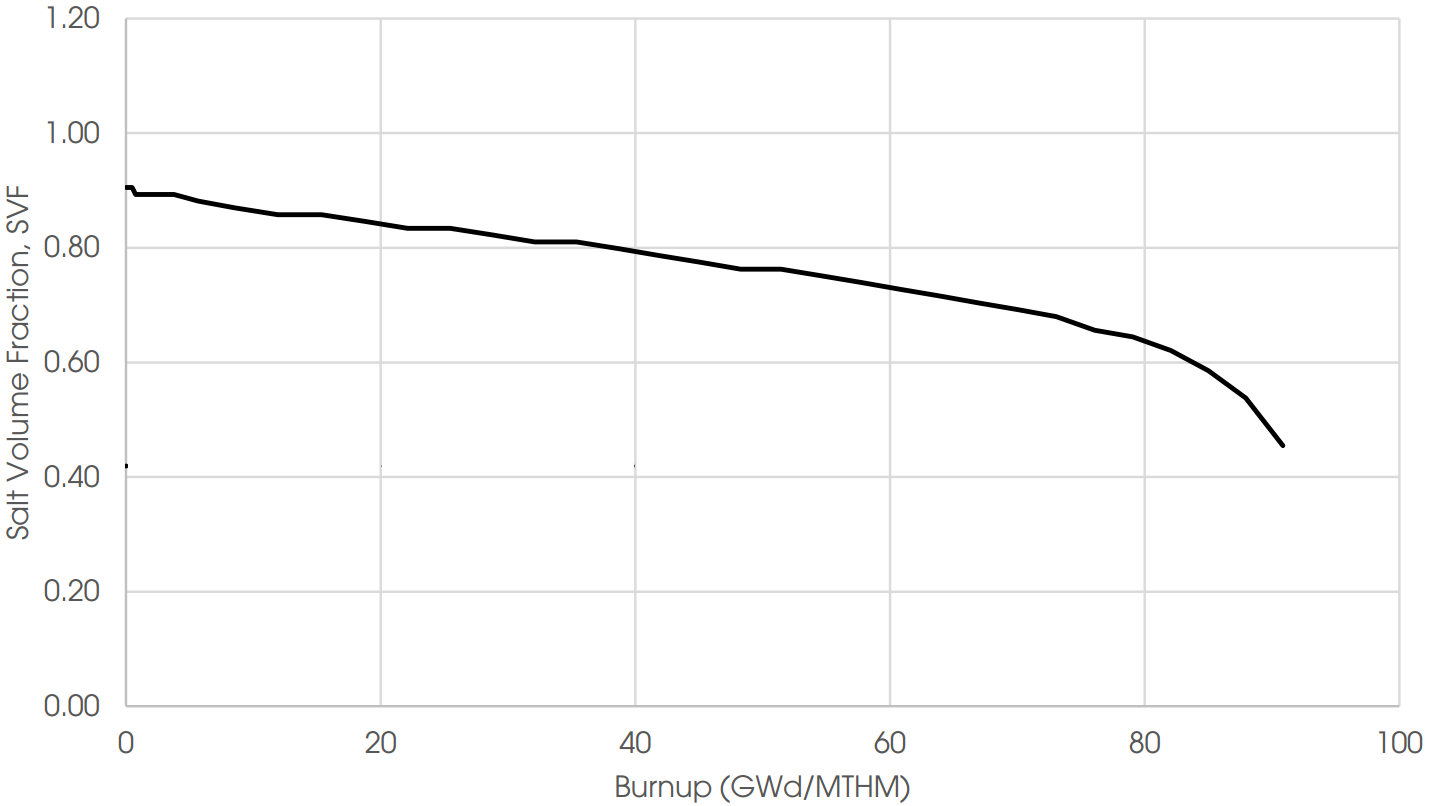
\includegraphics[width=\textwidth]{ch4/svf_predetermined.png}
	\caption{The change in SVF as a function of burnup in the \gls{TAP} 
	reactor (reproduced from Transatomic Power Neutronics Overview  
	\cite{transatomic_power_corporation_neutronics_2016}).}
	\label{fig:svf-predetermined}
\end{figure}


\subsection{Serpent 2 full-core model} \label{sec:tap_model}
Nest and lattice geometry types as well as universe transformation 
capabilities of Serpent \cite{leppanen_serpent_2014}  are employed to 
represent \gls{TAP} core. Figure~\ref{fig:tap-serpent-plan} shows the $XY$ 
section of whole-core configuration at the expected reactor operational level 
when all control rods are fully withdrawn. Figures~\ref{fig:tap-serpent-elev} 
and ~\ref{fig:tap-serpent-elev-zoom} show a longitudinal section of the 
reactor. This model contains the moderator rods with silicon carbide cladding, 
pressure vessel, and inlet and outlet plena (Table~\ref{tab:tap_model_param}). 
Fuel salt flows around rectangular moderator assemblies consisting of lattices 
of small-diameter zirconium hydride rods in a corrosion-resistant material. 
The salt volume fraction for Figure ~\ref{fig:tap-serpent-plan} is 0.917204, 
which means the modeled core is under-moderated and has intermediate neutron 
spectrum. Quarter-core configurations of the \gls{TAP} core with various salt 
volume fraction, used in the current work to maintain criticality for 
reasonable operational period ($>20$ years), are listed in 
Table~\ref{tab:tap_adjustable_core},Figures~\ref{fig:tap-406-681}, and 
\ref{fig:tap-840-1668} in Appendix~\ref{appex:geometries}.
\begin{figure}[htp!] % replace 't' with 'b' to 
	\centering
	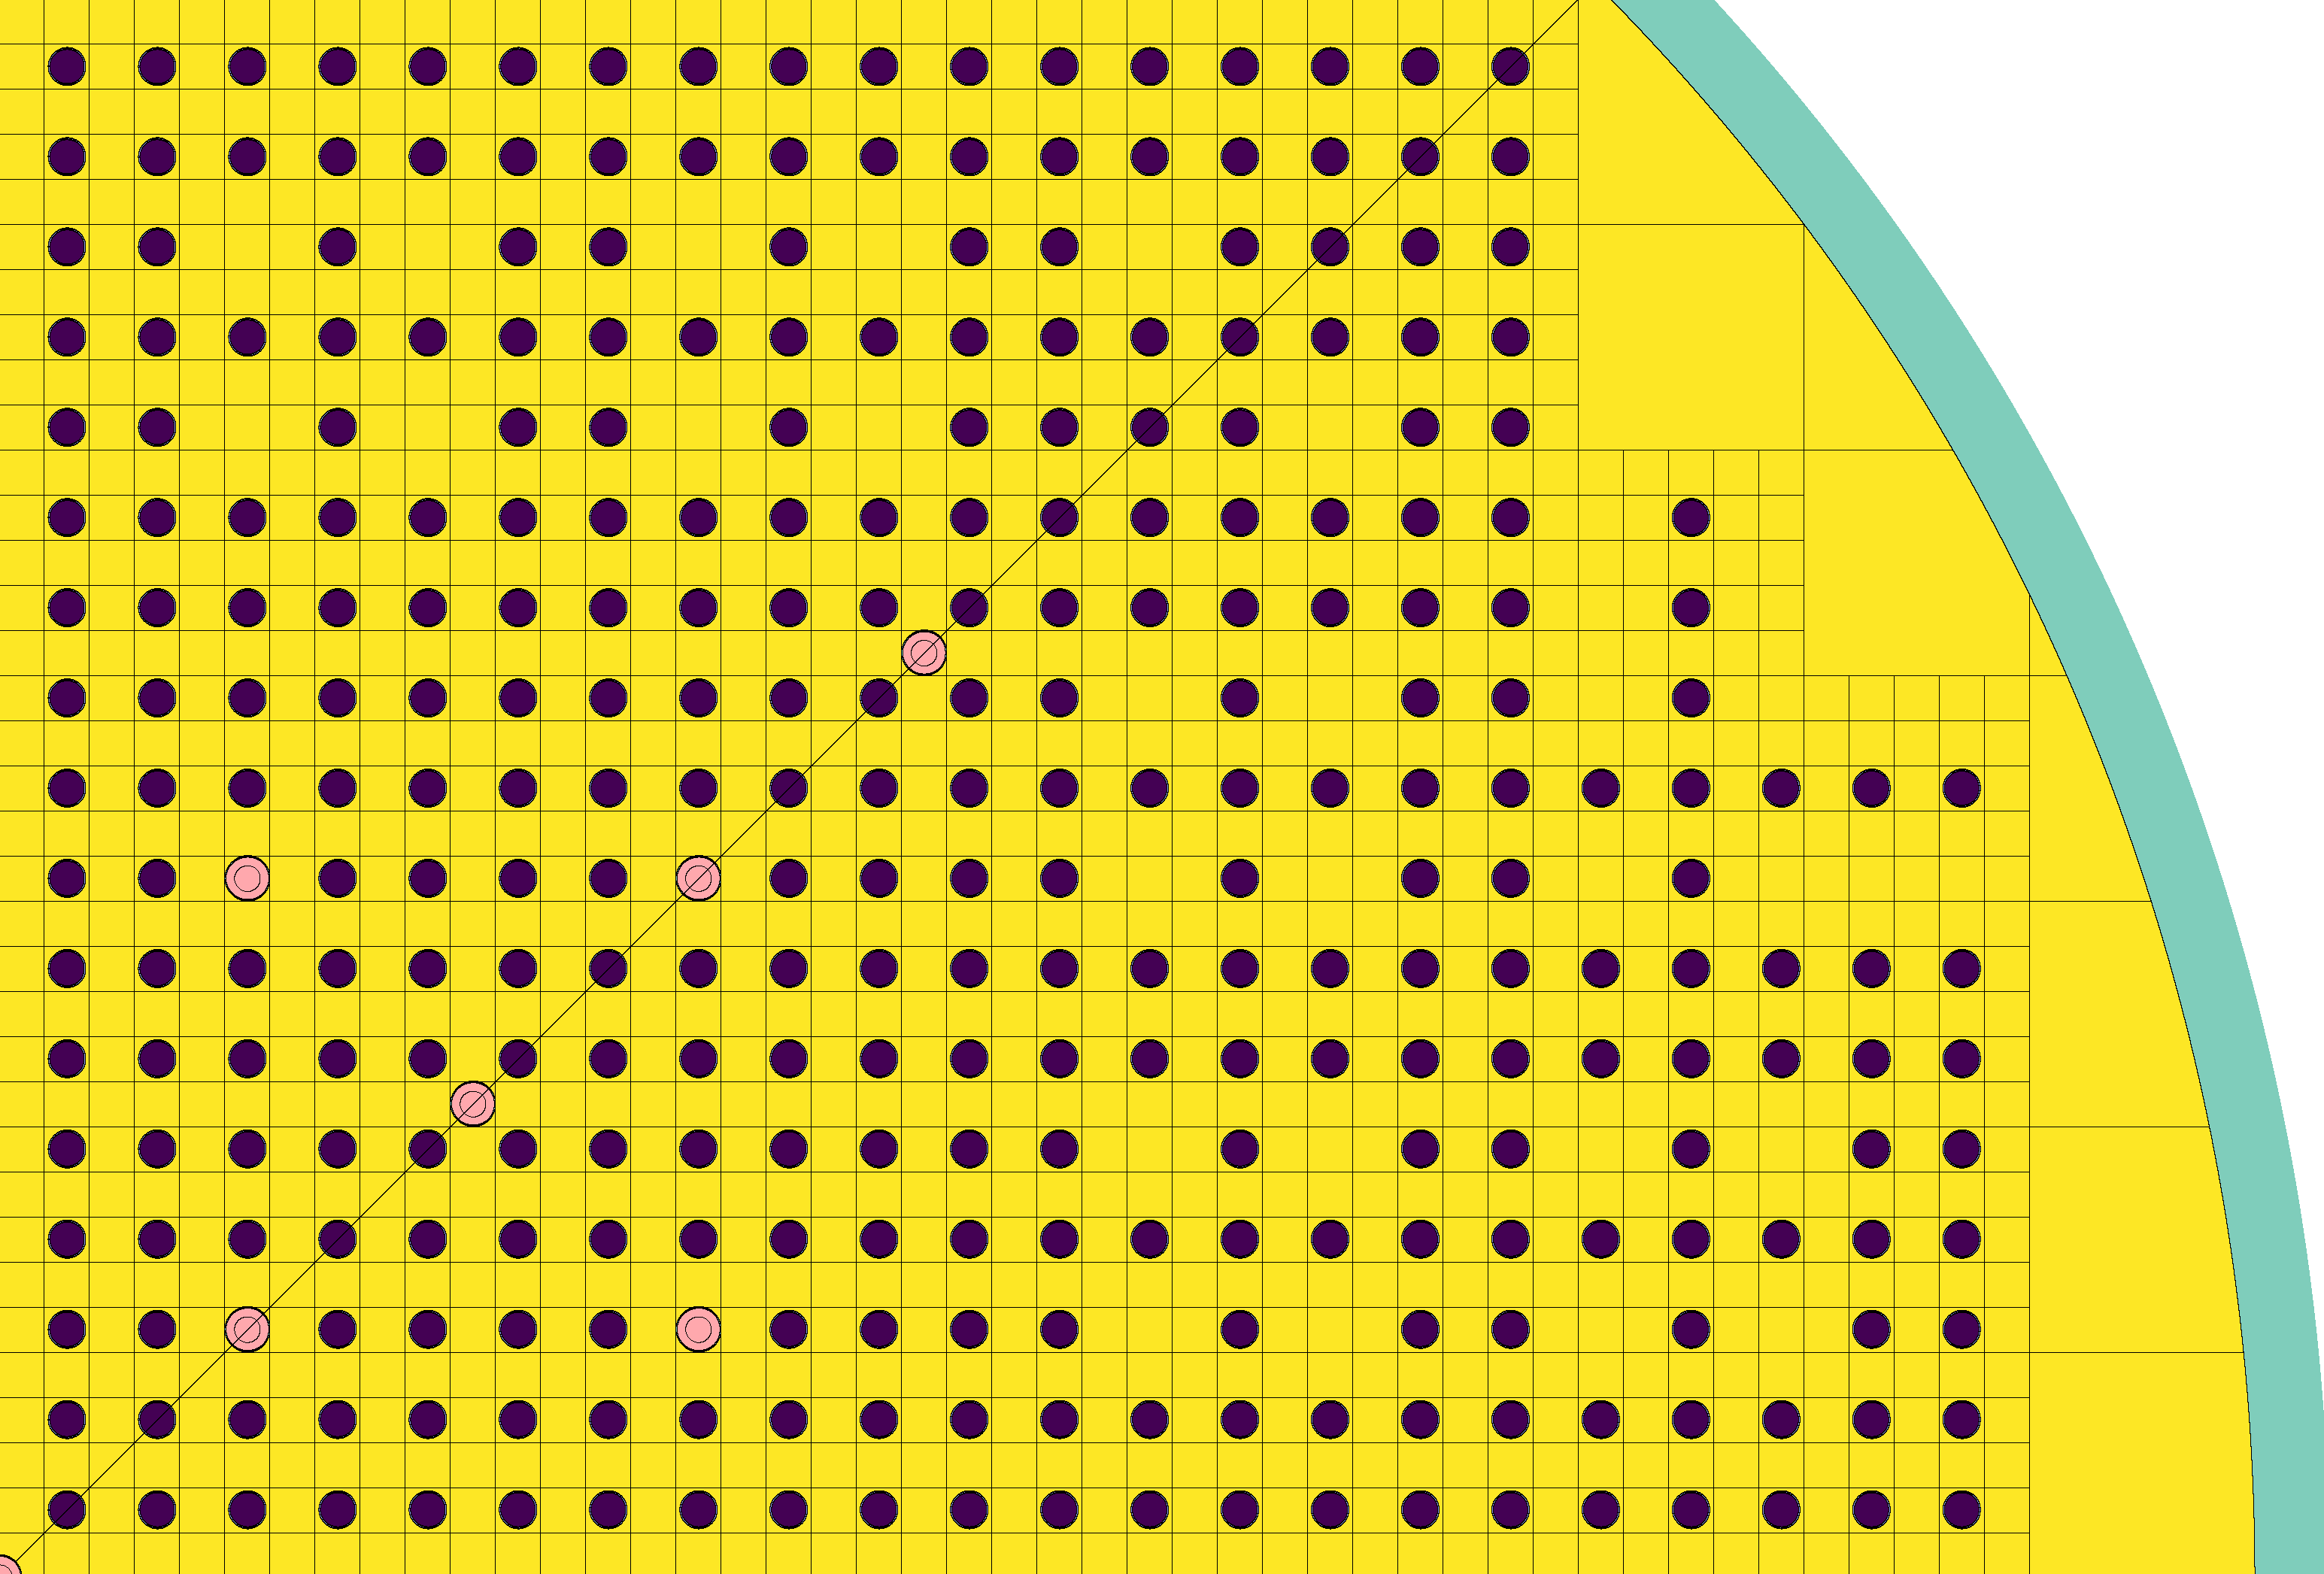
\includegraphics[width=0.75\textwidth]{ch4/tap_plan_view_serpent_347.png}
	\caption{An $XY$ section of the \gls{TAP} model at horizontal midplane 
		with fully withdrawn control rods at \gls{BOL} (347 moderator rods, 
		salt volume fraction is equal 0.917204). 
		The violet color represents zirconium hydride, and the yellow 
		represents fuel salt. 
		The blue color shows Hastelloy-N, a material used for the vessel wall, 
		and the pink color is the air.}
	\label{fig:tap-serpent-plan}
\end{figure}

\begin{figure}[htp!] % replace 't' with 'b' to 
	\centering
	
\includegraphics[width=0.6\textwidth]{ch4/tap_elev_view_serpent_347.png}
	\caption{45$^{\circ}$ $XZ$ section of the \gls{TAP} core model.}
	\label{fig:tap-serpent-elev}
\end{figure}

To represent the reactivity control system, the model has: 
\begin{enumerate}[label=(\alph*)]
	\item control rod guide tubes made of nickel-based alloy;
	\item control rods represented as a Boron Carbide (B$_4$C) cylinders 
	with a thin Hastelloy-N coating;
	\item air inside guide tubes and control rods;
\end{enumerate}
The control rods must be able to suppress excess reactivity at the \gls{BOL} 
when the core configuration is the most reactive and the neutron spectrum is 
the hardest. The control rod design shown on 
Figures~\ref{fig:tap-serpent-plan} and \ref{fig:tap-serpent-elev-zoom} is 
comprised of a cluster of 25 rods that provide a total reactivity worth of 
$4226\pm9pcm$ at the \gls{BOL}.

\begin{figure}[htp!] % replace 't' with 'b' to 
	\centering
	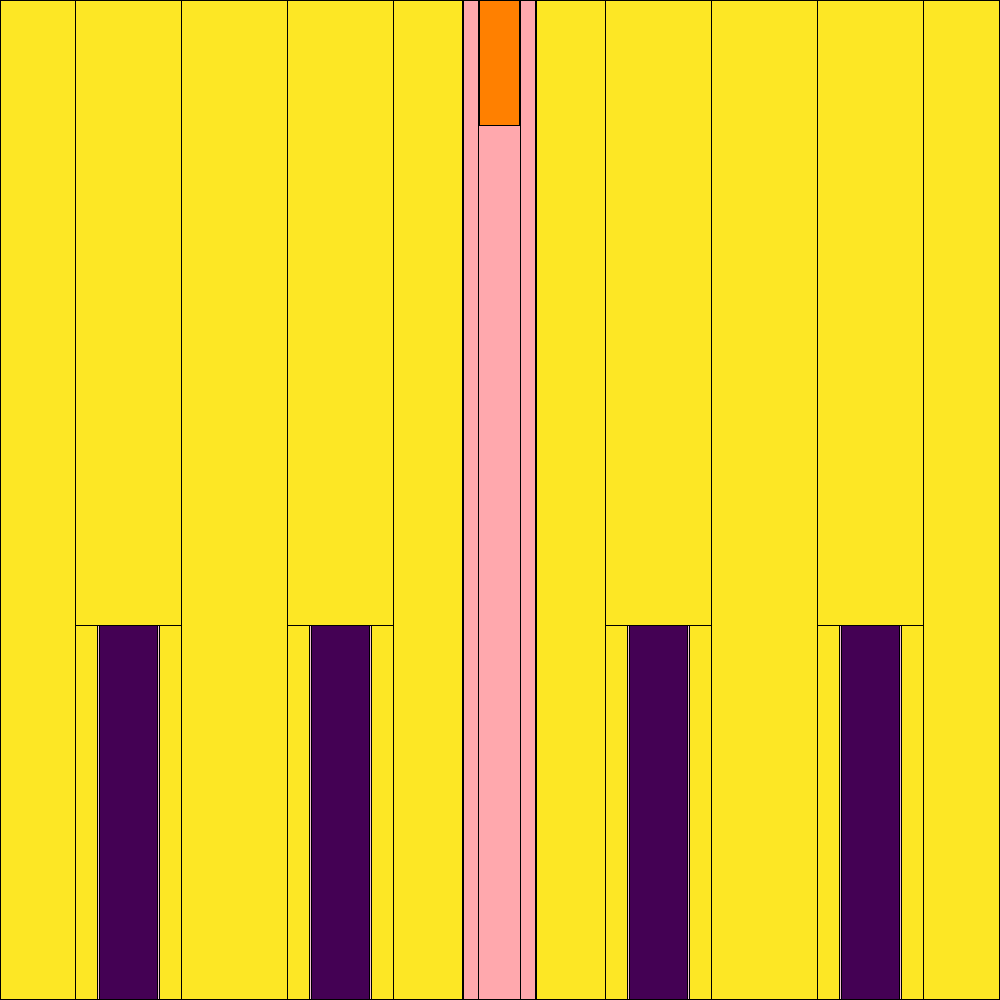
\includegraphics[width=0.55\textwidth]{ch4/tap_elev_view_zoomed_serpent.png}
	\caption{Zoomed $XZ$ section of the top of the moderator and control rods  
		in the \gls{TAP} model. The orange color shows Boron Carbide 
		(B$_4$C) absorbers used for control rods.}
	\label{fig:tap-serpent-elev-zoom}
\end{figure}
%%%%%%%%%%%%%%%%%%%%%%%%%%%%%%%%%%%%%%%%%%%%%%%%%%
\begin{table}[ht!]
	\caption{Geometric parameters for the full-core 3D model of the 
		\gls{TAP} (reproduced from Betzler \emph{et al.} 
		\cite{betzler_assessment_2017-1}). }
	\centering
	\begin{tabularx}{0.9\textwidth}{s s x p{0.14\textwidth}}
		\hline
		\textbf{Component}&\textbf{Parameter}&\textbf{Value}& \textbf{Unit}   
		\\ \hline
		\multirow{4}{*}{\begin{tabular}[c]{@{}l@{}}Moderator\\ 
				rod\end{tabular}} 
		& Cladding thickness      	  			    & 0.10 & cm				 
		\\  
		& Radius 				      	  			& 1.15 & cm				 
		\\  
		& Length				      	  			& 3.0  & m				 
		\\  
		& Pitch				      	  			& 3.0  & cm  			 \\ 
		\hline 
		
		\multirow{2}{*}{\begin{tabular}[c]{@{}l@{}}Moderator\\ 
				assembly\end{tabular}} 
		& Array				      	  			& 5 $\times$ 5 & 
		rods$\times$rods \\  
		& Pitch				      	  			& 15.0 & cm    				 
		\\  \hline
		
		\multirow{4}{*}{\begin{tabular}[c]{@{}l@{}}Core\end{tabular}}          
		& Assemblies  				   	  			& 268  & assemblies/core 
		\\  
		& Inner radius			      	  			& 1.5  & 
		m    				 \\  
		& Plenum height			   	  			& 25.0 & cm    				 
		\\  
		& Vessel wall thickness     	  			& 5.0 & 
		cm    				 \\ \hline            
	\end{tabularx}
	\label{tab:tap_model_param}
\end{table}
%%%%%%%%%%%%%%%%%%%%%%%%%%%%%%%%%%%%%%%%%%%%%%%%

The control rod cluster is modeled using the \textbf{TRANS} Serpent 2 feature, 
which allows the user to easily change the control rod position during the 
simulation. The current works assumed that all control rods are fully 
withdrawn from the core (Figure~\ref{fig:tap-serpent-elev-zoom}), but user can 
use SaltProc v1.0 reactivity control capabilities to change control 
rod position during operation. In this dissertation, all figures of the core 
were generated using the built-in Serpent plotter.


\subsection{TAP fuel salt reprocessing system}
The \gls{TAP} nuclear island contains a fission product removal system. 
Gaseous \glspl{FP} are continuously removed using an off-gas system while 
liquid and 
solid \glspl{FP} are extracted via a chemical processing system. As these 
byproducts are gradually removed, a small quantity of fresh fuel salt is 
regularly added to the primary loop. This process conserves a constant fuel 
salt mass and keeps the reactor critical. In contrast with the \gls{MSBR} 
reprocessing system, the \gls{TAP} design does not need a protactinium 
separation and isolation system because it operates in a uranium-based 
single-stage fuel cycle. The authors of the \gls{TAP} concept suggested three 
distinct fission product removal methods 
\cite{transatomic_power_corporation_neutronics_2016}:
\paragraph{Off-Gas System:} The off-gas system removes gaseous fission 
products such as krypton and xenon, which are then compressed and stored 
temporarily until they have decayed to the background radiation level. Trace 
amounts of tritium are also removed and bottled in a liquid form via the same 
process. Also, the off-gas system directly removes a small fraction of the 
noble metals.
\paragraph{Metal Plate-Out/Filtration:} A nickel mesh filter removes noble and 
semi-noble metal solid fission products as they plate out onto internal surface
of the filter.
\paragraph{Liquid Metal Extraction:} Lanthanides and other non-noble metals 
stay dissolved in the fuel salt. They generally have a lower capture cross 
section and thus absorb fewer neutrons than $^{135}$Xe, but their extraction 
is essential to ensure normal operation. In the \gls{TAP} reactor, lanthanide 
removal is accomplished via a liquid-metal/molten salt extraction process 
similar to that developed for \gls{MSBR} by \gls{ORNL}  
\cite{robertson_conceptual_1971}. The process converts the dissolved 
lanthanides into a well-understood oxide waste form, similar to that of 
\gls{LWR} \gls{SNF}. This oxide waste comes out of the \gls{TAP} reprocessing 
plant in ceramic granules and can be sintered into another convenient form for 
storage \cite{transatomic_power_corporation_technical_2016}.

Figure~\ref{fig:tap-reproc} shows the principal design of the \gls{TAP} 
primary loop, including an off-gas system, nickel mesh filter, and lanthanide 
chemical extraction facility. Similarly to the \gls{MSBR}, an off-gas system 
is also based on a simple process of helium sparging through fuel salt with 
consequent gas bubbles removed before returning the fuel salt to the core. 
Nevertheless, one crucial difference must be noted: the \gls{MSBR} gas 
separation system suggested helium injection and subsequent transport of the 
voids throughout the primary loop, including the core for at least ten full 
loops \cite{robertson_conceptual_1971}. It is a significant concern for safe, 
stable operation because the increase of void fraction in the fuel salt when 
it enters back to the core would cause unpredictable reactivity change. This 
drawback can be overcome by using an effective gas separator for stripping 
helium/xenon bubbles before returning the salt to a primary loop 
(Figure~\ref{fig:tap-reproc}, blue block). 
\begin{figure}[htp!] % replace 't' with 'b' to 
	\centering
	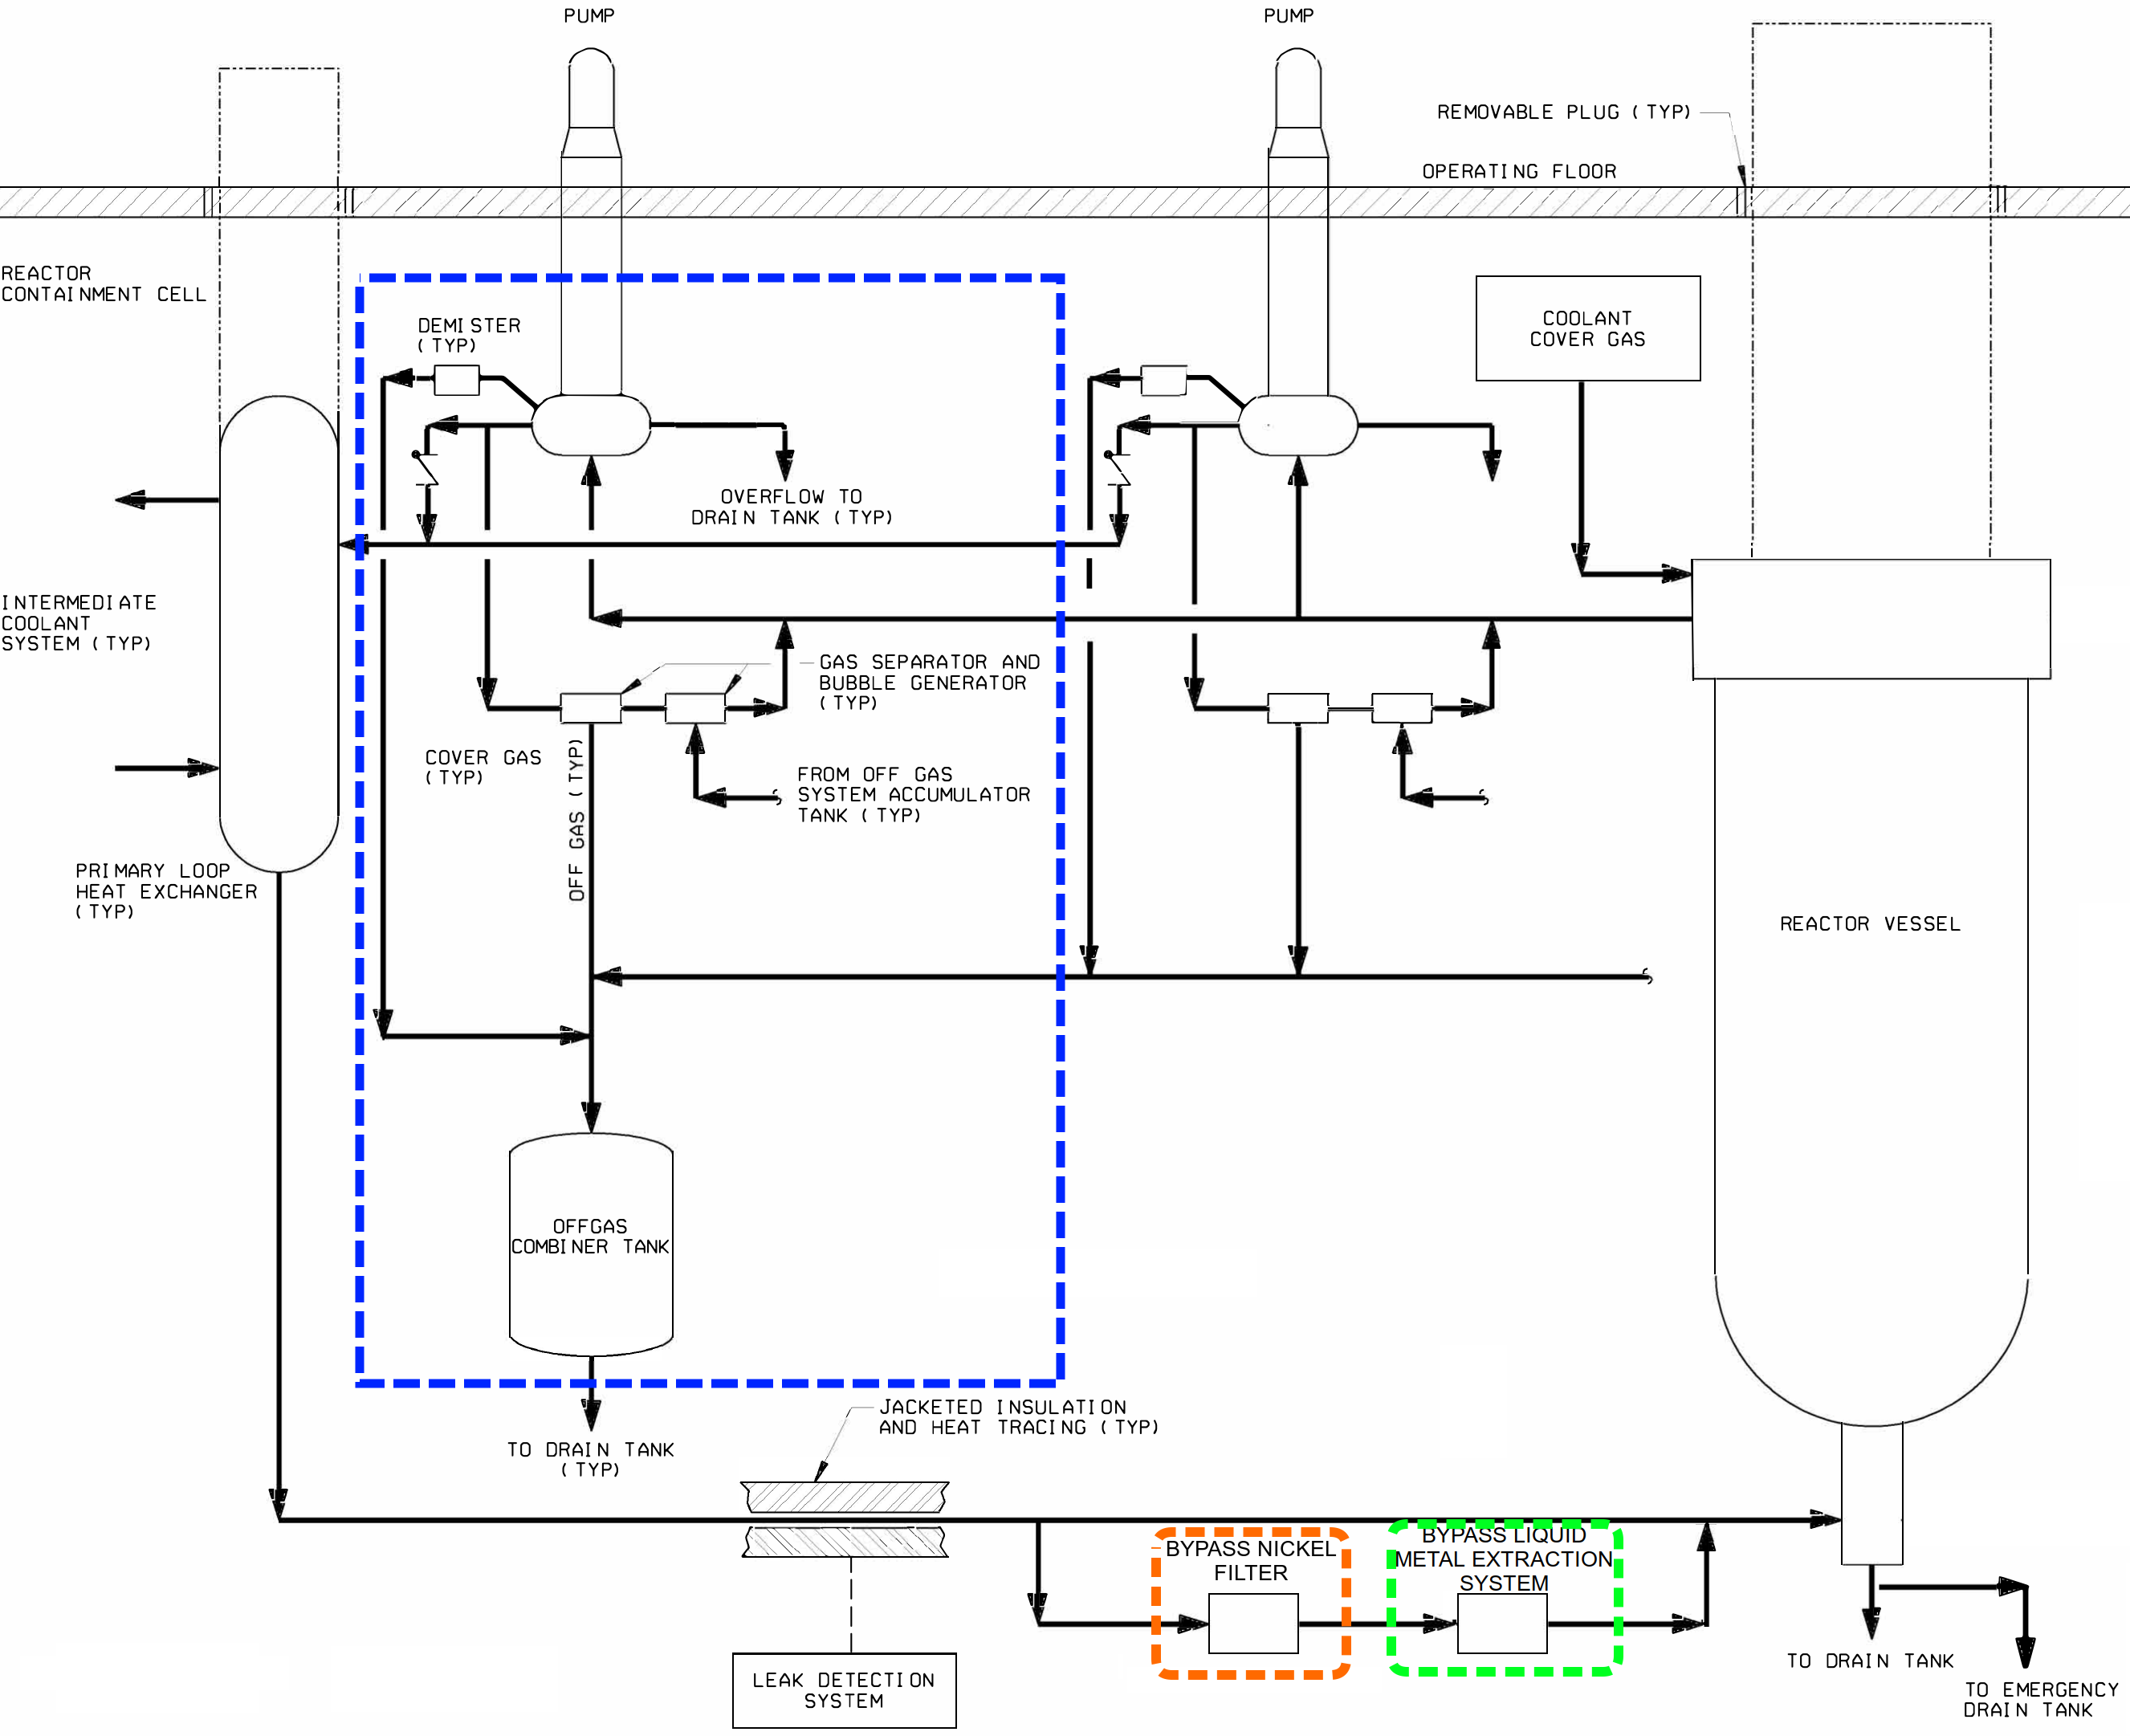
\includegraphics[width=\textwidth]{ch4/tap_primary_loop.png}
	\caption{Simplified \gls{TAP} primary loop design including off-gas system 
		(blue), 
		nickel filter (orange) and liquid metal extraction system (green) 
		(reproduced from \cite{transatomic_power_transatomic_2019}).}
	\label{fig:tap-reproc}
\end{figure}

Noble and semi-noble metal solid fission products tend to plate out onto metal 
surfaces including piping, heat exchanger tubes, reactor vessel inner surface, 
etc. Previous research by \gls{ORNL} \cite{robertson_conceptual_1971} reported 
that about 50\% of noble and semi-noble metals would plate out inside 
\gls{MSBR} systems without any special treatment. To improve the extraction 
efficiency of these fission products, the \gls{TAP} concept suggested 
employing a nickel mesh filter located in a bypass stream in the primary loop 
(Figure~\ref{fig:tap-reproc}, orange block). The main idea of this filter is 
to create a maze with large metal (nickel) surface area. The fuel salt is  
flowing throughout the filter and noble metals plate-out on the internal  
filter surface. 

This Liquid Metal Extraction process for the \gls{TAP} concept has been 
adopted from the \gls{MSBR}. The \gls{MSRE} demonstrated a liquid-liquid 
extraction process for removing rare earths and lanthanides from fuel salt and 
estimated efficiency of this process. Removal efficiency ($\epsilon_{RE}$) of  
this process is the function of salt mass flow rate, liquid bismuth mass 
flow rate, interfacial areas between salt and metal, and mass transfer 
coefficient for each noble metal species. The most recent research for LiF 
salt (for the \gls{MSFR} concept) reported the following form of extraction 
efficiency correlation \cite{rodrigues_actinide/lanthanide_2015}:
\begin{align} 
\epsilon_{RE} &= \frac{1}{1+10^{\lambda}} \nonumber \\
&= \frac{1}{1+10^{f(A, \dot{m}_{Bi}, \dot{m}_{salt}, N, K)}} \label{eq:re_eff}
\intertext{where}
A&= \mbox{metal-to-salt interface area} \nonumber \\
\dot{m}_{Bi}&= \mbox{bismuth mass flow rate} \nonumber \\
\dot{m}_{salt}&= \mbox{salt mass flow rate} \nonumber \\
N&= \mbox{number of stages} \nonumber \\
K&= \mbox{liquid phase mass transfer coefficient} \nonumber 
\end{align}
Correlations are different for various lanthanides and can be determined from 
experimental data and/or existing analytical models 
\cite{mcneese_engineering_1971, delpech_possible_2012, 
	rodrigues_actinide/lanthanide_2015}.

In fact, due to similarities in reprocessing schemes, the \gls{TAP} project 
reported almost the same set of elements for removal and similar effective 
cycle times as suggested for \gls{MSBR} (Table~\ref{tab:reprocessing_list}). 
The \gls{TAP} neutronics whitepaper specifies additional low-probability 
fission products and gases that should be removed during operation. These 
elements are categorized into the previously defined processing groups, but 
the removal rates of most of these elements (i.e., all except for hydrogen) 
are very low.

Details of gas removal and fuel reprocessing systems have historically 
been conceptual. Accordingly, liquid-fueled system designs including the 
\gls{TAP} concept usually assume ideal (rather than realistically constrained) 
removal efficiencies for reactor performance simulations. For the proposed 
work, a realistic online reprocessing system and reactor model will be created 
to capture the dynamics of fuel composition evolution during reactor 
operation. Gas removal efficiency will be represented in that model as a 
variable, described using mathematical correlation from Chapter 2 (see  
Equation~\ref{eq:gas_eff}). For the other \glspl{FP}, a fixed\footnote{ 
	Published information about dynamics of extraction efficiency during 
	reactor 
	operation for seminoble metals, volatile fluorides, and rare earths is 
	insufficient to inform a variable removal efficiency.}, non-ideal 
extraction efficiency based on cycle time from 
Table~\ref{tab:reprocessing_list} will be used in the fuel reprocessing model.

%%%%%%%%%%%%%%%%%%%%%%%%%%%%%%%%%%%%%%%%
\begin{table}[htbp!]
	\centering
	\caption{The effective cycle times for fission products removal  from the 
		\gls{TAP} reactor (reproduced from \cite{betzler_implementation_2017} 
		and 
		\cite{transatomic_power_corporation_neutronics_2016}).}
	\begin{tabular}{p{0.2\textwidth} p{0.42\textwidth} p{0.12\textwidth} 
			p{0.16\textwidth}}
		\hline 
		%\begin{tabularx}{\linewidth}{l X} \toprule 
		\textbf{Processing group} & \qquad\qquad\qquad \textbf{Nuclides} & 
		\textbf{Removal Rate (s$^{-1}$)} & \textbf{Cycle time (at full power)} 
		\\ [5pt] \hline 
		\multicolumn{3}{c}{\textit{Elements removed in \gls{MSBR} concept and 
				adopted for the \gls{TAP}} \cite{robertson_conceptual_1971}} \\
		Volatile gases & Xe, Kr								  & 5.00E-2 & 20 
		sec \\ [5pt]
		Noble metals & Se, Nb, Mo, Tc, Ru, Rh, Pd, Ag, Sb, Te & 5.00E-2 & 20 
		sec \\ [5pt]
		Seminoble metals & Zr, Cd, In, Sn	  				  & 5.79E-8 & 200 
		days \\ [5pt]
		Volatile fluorides & Br, I 							  & 1.93E-7 & 60 
		days \\ [5pt]
		Rare earths & Y, La, Ce, Pr, Nd, Pm, Sm, Gd           & 2.31E-7 & 50 
		days \\ [5pt]
		\qquad & Eu & 2.32E-8 & 500 days \\ [5pt]
		Discard & Rb, Sr, Cs, Ba & 3.37E-9 & 3435 days \\ [5pt] 
		\hline
		
		\multicolumn{3}{c}{\textit{Additional elements removed} 
			\cite{transatomic_power_corporation_neutronics_2016, 
				betzler_implementation_2017}  } \\
		Volatile gases & H								  	& 5.00E-2 & 20 
		sec    \\ [5pt]
		Noble metals & Ti, V, Cr, Cu						& 3.37E-9 & 3435 
		days \\ [5pt]
		Seminoble metals & Mn, Fe, Co, Ni, Zn, Ga, Ge, As   & 3.37E-9 & 3435 
		days \\ [5pt]
		Rare earths & Sc									& 3.37E-9 & 3435 
		days \\ [5pt]
		Discard & Ca										& 3.37E-9 & 3435 
		days \\ [5pt] 
		\hline
	\end{tabular}
	\label{tab:reprocessing_list}
	\vspace{-0.9em}
\end{table}
%%%%%%%%%%%%%%%%%%%%%%%%%%%%%%%%%%%%%%%%%%%%%%%%%%%%%%%%%%%%%%%%%%%%%%%%%%%%%%%



\section{Long-term depletion case demonstration and validation}
\subsection{Fuel salt isotopic composition dynamics}

\section{Reactor load following analysis}

\section{Prototype design for the xenon removal system}

\section{Concluding remarks}